\documentclass[12pt, twoside]{article}
\usepackage[letterpaper, margin=1in, headsep=0.5in]{geometry}
\usepackage[english]{babel}
\usepackage[utf8]{inputenc}
\usepackage{amsmath}
\usepackage{amsfonts}
\usepackage{amssymb}
\usepackage{tikz}

\usepackage{pgfplots}
\pgfplotsset{width=9cm,compat=1.9}

\usepackage{venndiagram}

\usepackage{graphicx}
\usepackage{enumitem}
\usepackage{multicol}

\usepackage{fancyhdr}
\pagestyle{fancy}
\fancyhf{}
\renewcommand{\headrulewidth}{0pt} % disable the underline of the header

\fancyhead[LE]{\thepage}
\fancyhead[RO]{\thepage \\ Name: \hspace{4cm} \,\\}
\fancyhead[LO]{BECA / Dr. Huson / IB Mathematics\\* Unit 4: Linear functions and regression\\* 3 January 2020}

\begin{document}
\begin{enumerate}
    \subsubsection*{Do Now: Graphing linear equations, tangent as slope}
    
    \item \begin{enumerate}
        \item Graph and label the two equations. Mark their intersection as an ordered pair.
          \begin{multicols}{2}
            $y =\frac{2}{3}x-4$ \\
            $4x+3y=6$ \hfill (4 pts)
          \end{multicols}     \vspace{1cm}
        \item Find the slopes of the two lines. \hfill (2 points)
          \begin{multicols}{2}
            $m_1=$ \\
            $m_2=$
          \end{multicols}
        \item Why is it incorrect to write $m_1=\frac{2}{3}x$? \hfill (1 point) \vspace{2cm}
        \item Are the lines parallel, perpendicular, or neither? Justify your answer with an equation or inequality using the slopes. \hfill (2 points)
        \vspace{2cm}
      \end{enumerate}
        \begin{center}
          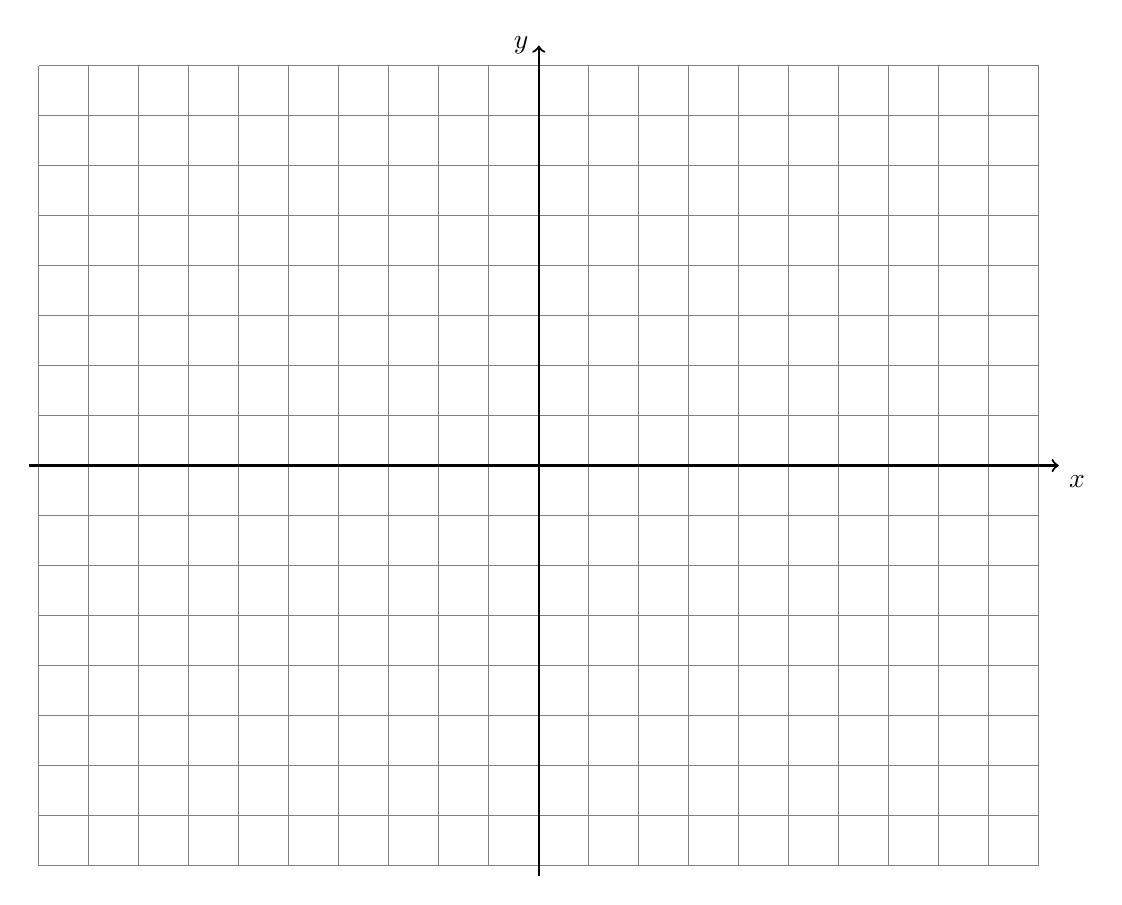
\begin{tikzpicture}[scale=.635]
            \draw [help lines] (-10,-8) grid (10,8);
            \draw [thick, ->] (-10.2,0) -- (10.4,0) node [below right] {$x$};
            \draw [thick, ->] (0,-8.2)--(0,8.4) node [left] {$y$};
          \end{tikzpicture}
        \end{center}
    
\newpage
    \item \begin{enumerate}
    \item Graph and label $\triangle ABC$ with $A(0,0)$, $B(7,4)$, and $C(7,0)$.
    \begin{center}
        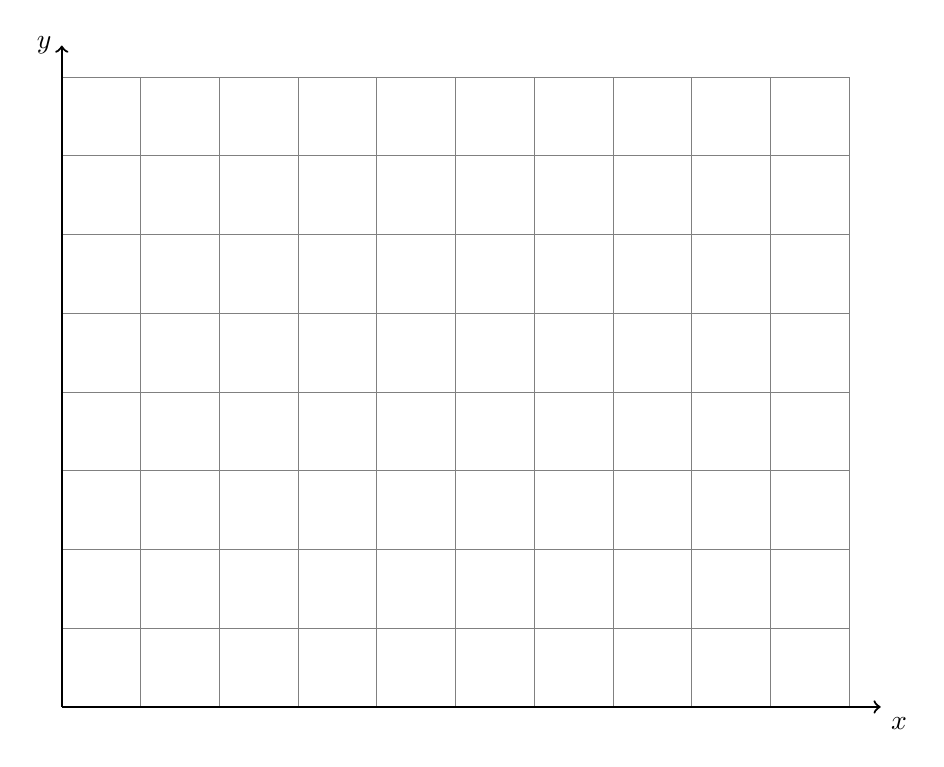
\begin{tikzpicture}%[scale=.635]
        \draw [help lines] (0,0) grid (10,8);
        \draw [thick, ->] (0,0) -- (10.4,0) node [below right] {$x$};
        \draw [thick, ->] (0,0)--(0,8.4) node [left] {$y$};
        \end{tikzpicture}
    \end{center}
    \item Find the slope and $y$-intercept of the line $\overleftrightarrow{AB}$.
        \begin{multicols}{2}
        $m_{AB}=$ \\
        $b_{AB}=$
        \end{multicols} \vspace{0.5cm}
    \item Write down the equation of each line. \\[0.5cm]
        $\overleftrightarrow{AB}$: \hfill
        $\overleftrightarrow{BC}$: \hfill
        $\overleftrightarrow{AC}$: \hspace{2cm}
    \vspace{2cm}
    \item Find the measure of $\angle BAC$ in degrees with a protractor. \vspace{0.5cm}
    \item Find the same $m\angle BAC$ with a calculator's inverse tangent function.\\[0.5cm]
    $\displaystyle \tan^{-1}(\frac{4}{7})=$
    \vspace{2cm}
    \end{enumerate}
    
\end{enumerate}
\end{document}